\section{Introduzione a UML}
\textbf{Unified Modeling Language} (UML) è un linguaggio standardizzato per il supporto alla descrizione e alla progettazione dei sistemi software.
Sebbene sia tendenzialmente utilizzato in contesti orientati agli oggetti, è possibile usufruirne anche per descrivere sistemi hardware o comprendere il
dominio operativo nel quale si lavora.\par
Presenta lo standard \textbf{Object Management Group} (OMG) e unifica in una singola collezione le varie notazioni pre-esistenti, integrandole e
rendendole orientate agli oggetti. Si tratta di un linguaggio per la \textbf{modellazione} usato spesso in ambito lavorativo da analisti e progettisti
software. Non è possibile usarlo per la programmazione. I tre utilizzi principali di UML riguardano: \begin{itemize}
	\item \textbf{Abbozzi}: Aiutano la comunicazione e la discussione, presentando solo le informazioni più importanti. Nella pratica sono usati tool
	come editor grafici o più direttamente una lavagna.
	\item \textbf{Progetti dettagliati}: Forniscono un modello completo da implementare mediante un modellatore UML, come Papyrus o Visual Paradigm.
	\item \textbf{Linguaggi di programmazione}: Meno comune dei due precedenti, è possibile usare dei tool appositi come UniMod per ottenere un modello
	eseguibile direttamente dalla composizione UML.
\end{itemize}
\noindent Esistono inoltre tre principali prospettive nell'utilizzo di UML: in primis, quella \textbf{concettuale}, che fornisce un punto di partenza
per lo sviluppo con la rappresentazione dei concetti del dominio operativo; in secundis, quella di \textbf{specifica}, che vede descritte nel diagramma
le interfacce del sistema senza dettagli implementativi; infine, la prospettiva di \textbf{implementazione} descrive gli elementi concreti del sistema
software, come le classi e gli attori.\par
I sistemi in UML sono destritti tramite le \textbf{viste}, intese come un particolare aspetto del software da un punto di vista di un ruolo specifico.
Lo scopo di un diagramma è la descrizione di una vista e il loro insieme compone il modello. Lo standard utilizzato in questo corso è UML 2.0, il quale
contiene 13 tipi di diagrammi diversi divisi in due macro-categorie: \textbf{diagrammi strutturali}, i quali descrivono la struttura statica del sistema
e \textbf{diagrammi comportamentali}, che rendono il comportamento dinamico.\par
UML è un linguaggio versatile; può essere utilizzato con qualsiasi processo nelle fasi di raccolta requisiti, design architetturale e delle componenti.
Per esempio, nella prima fase è possibile usare un use case diagram per la descrizione dei requisiti funzionali del sistema da una vista dell'utente.
\begin{figure}[h]
	\centering
	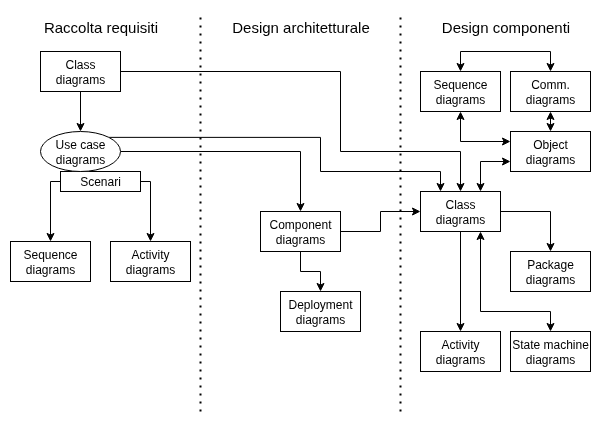
\includegraphics[width=1\linewidth]{Images/UML_diagrams_overview.png}
	\caption{Panoramica diagrammi UML 2.0}
\end{figure}

\noindent Non sempre è sufficiente l'implementazione dei diagrammi UML nel workflow; esistono due soluzioni principali per essere più esaustivi:
\textbf{non usare} UML oppure l'\textbf{estensione} del diagramma tramite \textbf{profili}, andando a sacrificare lo standard. Per quest'ultima
soluzione è possibile specificare particolari domini applicativi o tipi di applicazioni; un profilo è costituito principalmente da: \begin{itemize}
	\item \textbf{Stereotipi}: Elementi aggiuntivi ottenuti modificando quelli già esistenti.
	\item \textbf{Vincoli aggiuntivi}: Ulteriori restrizioni rispetto a quelle standard presenti in UML.
	\item \textbf{Informazioni semantiche aggiuntive}: Per dare ulteriori delucidazioni in merito agli elementi.
\end{itemize}
\noindent Quello di estendere i diagrammi rendendoli \textbf{illegali} è un compromesso utilizzato spesso in ambito lavorativo. Ciò fa capire quanto sia
fondamentale la flessibilità ai contesti rispetto all'attenersi esclusivamente agli standard e ai manuali. Lo sviluppo software è un processo creativo.
Divertiti.

%

\section{Diagrammi strutturali}
I \textbf{diagrammi di classe} definiscono le classi e relativi attributi, operazioni e relazioni con altre entità, come associazioni, aggregazioni,
composizioni, specializzazioni, generalizzazioni e dipendenze. Modellano quindi la parte strutturale (o statica) di un sistema software.\par
Il concetto di classe in UML è identico a quello presentato nel paradigma di orientamento agli oggetti; vengono rappresentare da un rettangolo diviso in
più compartimenti, i quali contengono nome, attributi e operazioni rispettivamente. Per quanto riguarda gli \textbf{attributi} presentano la segnatura:
\begin{center}
	visibilità nome: tipo [molteplicità] = default\{proprietà\}
\end{center}
\noindent Dove default è il valore base dell'attributo di un oggetto appena creato e proprietà definisce vincoli come sola lettura. Il nome è l'unica
parte obbligatoria da indicare, mentre le altre sono facoltative. Presentano inoltre quattro simboli corrispondenti ai modificatori di accesso, validi
anche per le operazioni, discusse più avanti: \begin{itemize}
	\item \textbf{Public}: +
	\item \textbf{Private}: -
	\item \textbf{Protected}: \#
	\item \textbf{Package private}: $\sim$
\end{itemize}
\noindent Anche la \textbf{molteplicità} è un dato che può presentare più valori e corrisponde a un quantitativo degli attributi, come per esempio le
dimensioni di una lista concatenata. Il valore di \textbf{default} è 1 e indica che nel software esiste una sola classe di questa fattura.
Alternativamente è possibile usare $0..1$ per dire \textbf{al più uno}, $0..*$ per \textbf{nessuno o numero imprecisato}, $1..*$ per \textbf{almeno uno},
oppure per generalizzare, usare $n,m$, definendo i loro valori. Le \textbf{operazioni} invece presentano la segnatura: \begin{center}
	visibilità nome(parametri): tipo-ritornato\{proprietà\}
\end{center}

\noindent Le \textbf{operazioni} presentano una segnatura simile a quella degli attributi, ma sono capaci di ricevere dei parametri all'interno delle
parentesi tonde. Sarà necessario dar loro una direzione con una freccia per permettere il collegamento fra le classi. Inoltre, essendo che è
comune prassi la scrittura di metodi getter e setter, generalmente sono omessi dallo spazio apposito.\par
In UML esistono due tipi di operazioni: le \textbf{query}, le quali ottengono un valore da un oggetto senza effetti secondari, e i \textbf{modificatori},
che modificano lo stato dell'oggetto su cui sono chiamate.\par
Per una migliore specifica, si fornisce il concetto di \textbf{datatype}, equivalente ad un valore definito dall'utente; possono essere una data o un
valore in Euro, per esempio. Si rappresentano come classi alle quali è aggiunto lo stereotipo $<<$datatype$>>$.\newline

\noindent Naturalmente, le classi possono essere messe in relazione. Il meccanismo è ottenuto tramite \textbf{associazioni}, annotate tramite frecce
che mostrano la direzione con la quale deve essere letta la relazione. Per esempio, se una classe "Person" ha una freccia uscente che entra nella
classe "car", significa che è possibile ottenere informazioni riguardo l'automobile a partire dalla persona.\par
Inoltre, è possibile porre una molteplicità alle associazioni, mostrando quanti oggetti possono esistere durante l'esecuzione del software con metriche
identiche a quelle discusse in precedenza. Attributi e associazioni sono due modi per rappresentare la stessa cosa, ma per convenzione si usano i primi
per campi di tipi primitivi e datatype, mentre le seconde se il tipo è definito da una classe.\par
Con lo scopo di rendere ulteriormente comprensibile un class diagram è possibile integrarlo tramite gli \textbf{object diagram}, rappresentanti le
istanze di una classe, spiegando anche la relazione tra classe e oggetti mediante l'operazione $<<$istanzia$>>$. È possibile segnalare operazioni e
attributi statici sottolineandoli.\par
Altre casistiche possibili nella scrittura dei diagrammi di classe o di oggetti sono le \textbf{associazioni riflessive}, dove una classe ha
un'associazione con sé stessa, le \textbf{classi associative}, dove le proprietà appartengono all'associazione piuttosto che alle classi, le \textbf{
associazioni bidirezionali}, che rendono le informazioni reperibili da entrambe le classi coinvolte e richiedono una sincronizzazione quando vengono
istanziate, le \textbf{aggregazioni}\footnote{Consigliabile utilizzarle solo a livello concettuale. In ambito concreto possono confondersi con le
associazioni.}, con le quali è possibile rappresentare la relazione fra un insieme e una delle sue parti con un rombo alla base della freccia, le
\textbf{composizioni}, forme più rigorose delle aggregazioni, dove se è deallocato il composto, allo stesso modo seguiranno le sue parti.\par
Abbiamo infine tre concetti molto più vicini alla programmazione orientata agli oggetti, come la \textbf{generalizzazione ed ereditarietà}; un
meccanismo grazie al quale elementi specializzati incorporano struttura e comportamento di elementi più generali. Inoltre, è possibile segnalare le
\textbf{dipendenze} tra le classi con una freccia tratteggiata; in loro presenza, la modifica di una classe ne comporta una anche nell'altra. Esistono
degli stereotipi appositi, come $<<use>>$, $<<call>>$ e $<<create>>$.

\begin{figure}[h]
	\centering
	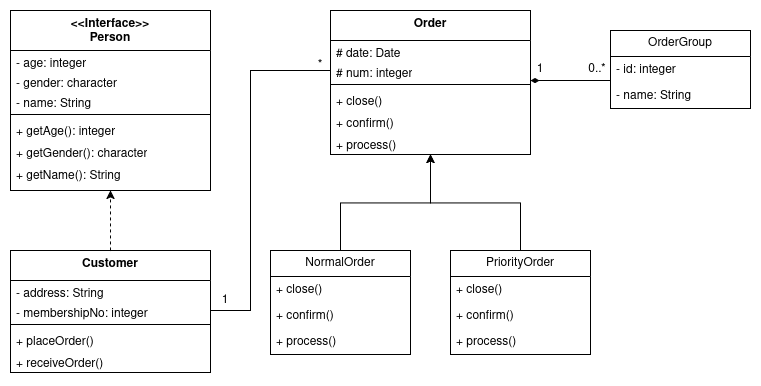
\includegraphics[width=0.9\linewidth]{Images/classDiagramExample.png}
	\caption{Esempio class diagram}
\end{figure}

\noindent Introduciamo ora il concetto di \textbf{interfaccia}, inteso come l'insieme delle operazioni visibili all'esterno degli oggetti, istanze di
quella classe. Si tratta di un'entità priva di implementazione simile a una classe, definita con classi concrete che fanno uso della sua struttura.
La relazione è generalmente indicata con frecce tratteggiate verso la classe interfaccia, la quale conterrà lo stereotipo $<<$interface$>>$.\par
In alternativa, è possibile usare la notazione \textbf{lollipop}, dove due classi sono collegate con una linea retta, al cui centro è presente un
cerchio (lollipop) che indica il nome dell'interfaccia richiesta, e un semicerchio (socket), che indica la classe richiedente.
	
\begin{figure}[h]
	\centering
	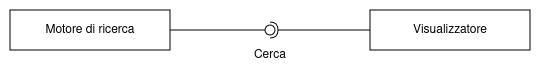
\includegraphics[width=0.7\linewidth]{Images/interfaceExample.png}
	\caption{Esempio interfaccia}
\end{figure}
	
\noindent Il vantaggio principale che si ottiene utilizzando interfacce è una diminuzione dell'accoppiamento tra classi; se durante la scrittura del
codice si nota che più classi utilizzano meccanismi simili, potrebbe essere corretto astrarli con un'interfaccia e definire i metodi nelle classi
concrete\footnote{Questo è un esempio di un design pattern chiamato Strategy.}.\par
In generale, le associazioni, gli attributi e le generalizzazioni sono costrutti base per esprimere vincoli, ma non sempre bastano a rappresentarli
correttamente. Per questa ragione UML permette di specificarne ulteriori utilizzando il linguaggio naturale o un
\textbf{Object Constraint Language}\footnote{È un linguaggio usato anche per la specifica di pre e post-condizioni} (OCL), basato sulla logica del primo
ordine.

%

\section{Diagrammi di interazione}

\begin{figure}[h]
	\centering
	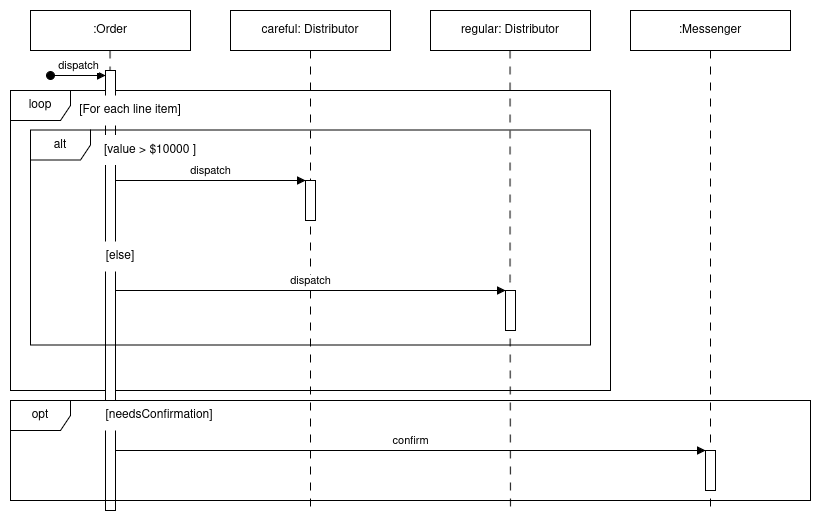
\includegraphics[width=0.9\linewidth]{Images/sequenceDiagramExample.png}
	\caption{Esempio sequence diagram}
\end{figure}

\begin{comment}
	Lez11 - 16/04/26 softEng
	
	--- Sequence diagram e communication diagram
	
	I diagrammi di interazione descrivono la collaborazione di un gruppo di oggetti (scambio di messaggi).
	I messaggi possono presentarsi in tre modi:
	- sincroni: Il mittente si pone in attesa del risultato
	- Asincroni: Il mittente continua l'esecuzione; questi ultimi sono usati per rappresentare i processi concorrenti.
	- trovati: messaggi il cui partecipante che lo genera è omesso
	Per scambiare messaggi è necessario avere una relazione tra le classi.
	
	La notazione del sequence diagram presenta due attori principali detti partecipanti (sarebbero le classi) indicate con tre segnature possibili:
	[nomeClasse]: oggetto di nome nomeClasse non specificando il tipo
	[:nomeClasse]: istanza anonima di nomeClasse
	[s:nomeClasse]: istanza di nomeClasse chiamata s
	Messaggi sincroni inficati con frecce piene; la risposta con una freccia tratteggiata.
	Naturalmente coi messaggi è possibile specificarne anche i parametri, con segnatura [returnValie = message(params): returnType]
	
	I messaggi possono essere anche usati per la creazione di istanze; allora la risposta andrà dentro ad un oggetto creato. Per indicare invece che la vita di un oggetto termina, si usa una risposta che entra in una X. Un oggetto si può anche autodistruggere.
	Cicli e condizioni possono essere espressi con i frame di interazione; cornici per inquadrare una parte del diagramma. Il primo operatore è loop, il secondo invece è opt, per optional. Un terzo si chiama Alt, per alternate e si usa per gli if-else.
	Naturalmente è possibile annidare i frame, sebbene faccia schifo a vedersi.
	Ref è invece usato per semplificare i sequence diagram; indica una reference ad un metodo specifico. Al posto di indicare l'intero diagramma coi messaggi, si usa il nome accerchiato dal frame ref.
	L'ultimo operatore è par, sta per parallel e indica metodi eseguiti concorrentemente. Naturalmente non ha senso accerchiare un solo metodo con par.
	
	I SD sono un buon mezzo per visualizzare l'interazione tra oggetti astrattamente, non la logica di controllo. Rendono chiare le chiamate e le relazioni tra le classi. Sconsigliato usare i frame di interazione; per la logica di controllo usare pseudocodice.
	Normalmente gli SD sono usati a due livelli differenti: a livello di requisiti per spiegare gli use case e il funzionamento astratto, e a livello di design, per descrivere più facilmente le relazioni tra le classi e il modo in cui interagiscono.
	Un diagramma di sequenza di sistema illustra invece gli eventi di I/O del sistema relativi ad uno scenario o più di uno use case. Hai praticamente lo use case ed il flusso dei messaggi è descritto tramite SD.
	
	--- Diagrammi di interazione
	Simile ai sequence diagram, condivide la sintassi, ma si rappresentano i messaggi come etichette degli archi con una direzione. Semplifica la struttura del diagramma rispetto a prima.
	
	--- Esercizio (ordine)
	Supponiamo di avere un ordine di acquisto; ci serve un'operazione per calcolare l'importo totale scontato con o.calcolaPrezzo().
	Per farlo l'ordine deve determinare l'importo di tutti i suoi elementi di linea [Quantità*prezzoUnitario]; dopo aver calcolato il totale l'ordine deve calcolare uno sconto globale che dipende dal cliente e scalarlo.
	
	Dunque o.calcolaPrezzo = totale-sconto
\end{comment}

%

\section{State Machine Diagram}

\begin{comment}
	Lez13 - 23-04-26 softEng
	
	# Prossima lezione il 6 maggio
	
	--- State machine diagrams
	Diagrammi che descrivono il comportamento di un componente, in termini di variazione del suo stato interno quando riceve un input di qualche tipo. Modello FSM, in pratica. Uno stato rappresenta una situazione nella vita di un oggetto durante la quale sono soddisfatte determinate condizioni e possono essere eseguite delle attività. Si cambia stato in base agli input ricevuti dagli attori.
	Si rappresenta come una FSM (ma dai?) e sugli archi stanno descritti eventi e input.
	Una FSM è sempre associata a un'entita e ne descrive il relativo comportamento. Riceve eventi che sono salvati su una coda ed estratti uno alla volta; la semantica è di tipo run-to-completion, quindi un evento è estratto solo dopo che è stato estratto il precedente.
	Inoltre, se ci sono più transazioni eseguibili in un dato momento (non determinismo se due transizioni dallo stesso stato con stesso evento e due condizioni diverse sono entrambe vere) ne viene eseguita solo una.
	Pallino nero è stato iniziale, nodi sono gli altri stati, archi son le transizioni. Un pallino nero accerchiato è lo stato finale e indica che l'esecuzione è terminata. Possono essercene più di uno.
	
	Le transizioni specificano come si passa tra gli stati. Specifica evento (trigger che attiva il passaggio), guardia (condizione che se vera permette il passaggio di stato) e attività (una o più azioni che sono compiute prima di cambiare stato). Transizione avviene come risposta a un evento. Eventi guardie e attività sono opzionali.
	
	Possiamo associare le FSM a una classe o un singolo oggetto per la durata del suo ciclo di vita.
	
	Ci sono più tipi di evento. Il primo è la ricezione di un messaggio, ma può esserci anche un evento di cambiamento (quando condizione passa da falsa a vero) o un evento temporale (si verifica dopo un tempo t o a una data precisa); si indica con when(condizione) nell'arco.
	Uno stato può reagire ad eventi e compiere attività anche senza una transizione ad uno stato diverso. Si possono mostrare nel secondo slot e seguono la sintassi delle transizioni. In particolare, entry ed exit sono attività speciali che si attivano ogni volta che si entera/escher dallo stato.
	Esiste anche do-activity che è eseguita mentre l'oggetto è nello stato. Può durare per un intervallo di tempo ed essere interrotta da altri eventi.
	
	Uno stato può essere semplice o composito. Quest'ultima forma consente di suddividere la complessità del modello. Nel senso, hai il macro-stato e una fsm interna. Si usa un'icona per rappresentare uno stato composito il cui comportamento interno non è mostrato.
	Possibile indicare concorrenza negli stati compositi aggiungendo slot alla macro-fsm.
	
	Entry ed exit points si indicano con cerchi bianchi e cerchi bianchi con una X all'interno rispettivamente.
	
	Quando è corretto usare le FSM? Per entità con una logica interna complessa.
	
	State machine si implementa in tre modi: switch case, con un design pattern state (ogni stato è una classe, si usa il polimorfismo per variare il comportamento) o delle STT con un tool che traduce da linguaggio apposito.
\end{comment}
